\begin{Exercise}[title=Suspension de voiture]
Une automobile est sommairement modélisée par une masse $m$ placée en $M$ et reposant sur une roue de centre $O$, par l’intermédiaire d’un ressort de raideur $k$ mis en parallèle sur un amortisseur de coefficient de frottement $h$.
En toutes circonstances, l’axe OM reste vertical.On se propose d’examiner le comportement du véhicule lorsqu’il a la vitesse $v$ sur une route dont le profil impose au centre O de la roue une élongation:
\[ z_0(x) = a\cos\left( \frac{2\pi x}{\lambda} \right) \]
par rapport à  son niveau d'équilibre.
On repère le mouvement de la masse par son élongation$ z(t)$ par rapport à sa position d’équilibre
quand le véhicule est au repos.
	\begin{center}
	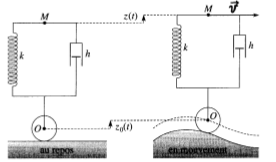
\includegraphics[scale=0.8]{../fig/suspension.png}
	\end{center}
\Question Établir l’équation différentielle en $z(t)$ du mouvement de la masse , lorsque le véhicule se déplace à vitesse constante $v$
\Question Déterminer l’amplitude du mouvement d’oscillation vertical du véhicule en régime permanent.
\Question À quelle allure convient-il de rouler pour que cette amplitude soit aussi faible que possible ?
\end{Exercise}
\begin{Answer}
	\Question $mz'' = -mg -k(z-z_0)-h(z'-z_0')$
	\Question On fais l'hypothèse d'une solution de meme forme que le second membre, à la pulsation $w=\frac{2\pi v}{\lambda}$ On réintroduit et on a pour une amplitude maximale:
	$A =\frac{g}{\omega^2+\omega_0^2} $ avec $\omega_0 = \sqrt{\frac{k}{m}}$
	\Question On ne veux pas $v$ tel que $\omega = \omega_0$ !
\end{Answer}
